% Options for packages loaded elsewhere
% Options for packages loaded elsewhere
\PassOptionsToPackage{unicode}{hyperref}
\PassOptionsToPackage{hyphens}{url}
\PassOptionsToPackage{dvipsnames,svgnames,x11names}{xcolor}
%
\documentclass[
  letterpaper,
]{article}
\usepackage{xcolor}
\usepackage{amsmath,amssymb}
\setcounter{secnumdepth}{5}
\usepackage{iftex}
\ifPDFTeX
  \usepackage[T1]{fontenc}
  \usepackage[utf8]{inputenc}
  \usepackage{textcomp} % provide euro and other symbols
\else % if luatex or xetex
  \usepackage{unicode-math} % this also loads fontspec
  \defaultfontfeatures{Scale=MatchLowercase}
  \defaultfontfeatures[\rmfamily]{Ligatures=TeX,Scale=1}
\fi
\usepackage{lmodern}
\ifPDFTeX\else
  % xetex/luatex font selection
\fi
% Use upquote if available, for straight quotes in verbatim environments
\IfFileExists{upquote.sty}{\usepackage{upquote}}{}
\IfFileExists{microtype.sty}{% use microtype if available
  \usepackage[]{microtype}
  \UseMicrotypeSet[protrusion]{basicmath} % disable protrusion for tt fonts
}{}
\makeatletter
\@ifundefined{KOMAClassName}{% if non-KOMA class
  \IfFileExists{parskip.sty}{%
    \usepackage{parskip}
  }{% else
    \setlength{\parindent}{0pt}
    \setlength{\parskip}{6pt plus 2pt minus 1pt}}
}{% if KOMA class
  \KOMAoptions{parskip=half}}
\makeatother
% Make \paragraph and \subparagraph free-standing
\makeatletter
\ifx\paragraph\undefined\else
  \let\oldparagraph\paragraph
  \renewcommand{\paragraph}{
    \@ifstar
      \xxxParagraphStar
      \xxxParagraphNoStar
  }
  \newcommand{\xxxParagraphStar}[1]{\oldparagraph*{#1}\mbox{}}
  \newcommand{\xxxParagraphNoStar}[1]{\oldparagraph{#1}\mbox{}}
\fi
\ifx\subparagraph\undefined\else
  \let\oldsubparagraph\subparagraph
  \renewcommand{\subparagraph}{
    \@ifstar
      \xxxSubParagraphStar
      \xxxSubParagraphNoStar
  }
  \newcommand{\xxxSubParagraphStar}[1]{\oldsubparagraph*{#1}\mbox{}}
  \newcommand{\xxxSubParagraphNoStar}[1]{\oldsubparagraph{#1}\mbox{}}
\fi
\makeatother


\usepackage{longtable,booktabs,array}
\usepackage{calc} % for calculating minipage widths
% Correct order of tables after \paragraph or \subparagraph
\usepackage{etoolbox}
\makeatletter
\patchcmd\longtable{\par}{\if@noskipsec\mbox{}\fi\par}{}{}
\makeatother
% Allow footnotes in longtable head/foot
\IfFileExists{footnotehyper.sty}{\usepackage{footnotehyper}}{\usepackage{footnote}}
\makesavenoteenv{longtable}
\usepackage{graphicx}
\makeatletter
\newsavebox\pandoc@box
\newcommand*\pandocbounded[1]{% scales image to fit in text height/width
  \sbox\pandoc@box{#1}%
  \Gscale@div\@tempa{\textheight}{\dimexpr\ht\pandoc@box+\dp\pandoc@box\relax}%
  \Gscale@div\@tempb{\linewidth}{\wd\pandoc@box}%
  \ifdim\@tempb\p@<\@tempa\p@\let\@tempa\@tempb\fi% select the smaller of both
  \ifdim\@tempa\p@<\p@\scalebox{\@tempa}{\usebox\pandoc@box}%
  \else\usebox{\pandoc@box}%
  \fi%
}
% Set default figure placement to htbp
\def\fps@figure{htbp}
\makeatother





\setlength{\emergencystretch}{3em} % prevent overfull lines

\providecommand{\tightlist}{%
  \setlength{\itemsep}{0pt}\setlength{\parskip}{0pt}}



 



\begin{titlepage}
    \centering
    \vspace*{5cm}
    {\Large Universidade CEUB \par}
    {\large Projeto Integrador III \par}
    \vfill
    {\large Nome da Equipe ou Aluno \par}
    {\large Brasília \par}
    {\large 2025 \par}
\end{titlepage}
\makeatletter
\@ifpackageloaded{bookmark}{}{\usepackage{bookmark}}
\makeatother
\makeatletter
\@ifpackageloaded{caption}{}{\usepackage{caption}}
\AtBeginDocument{%
\ifdefined\contentsname
  \renewcommand*\contentsname{Table of contents}
\else
  \newcommand\contentsname{Table of contents}
\fi
\ifdefined\listfigurename
  \renewcommand*\listfigurename{List of Figures}
\else
  \newcommand\listfigurename{List of Figures}
\fi
\ifdefined\listtablename
  \renewcommand*\listtablename{List of Tables}
\else
  \newcommand\listtablename{List of Tables}
\fi
\ifdefined\figurename
  \renewcommand*\figurename{Figure}
\else
  \newcommand\figurename{Figure}
\fi
\ifdefined\tablename
  \renewcommand*\tablename{Table}
\else
  \newcommand\tablename{Table}
\fi
}
\@ifpackageloaded{float}{}{\usepackage{float}}
\floatstyle{ruled}
\@ifundefined{c@chapter}{\newfloat{codelisting}{h}{lop}}{\newfloat{codelisting}{h}{lop}[chapter]}
\floatname{codelisting}{Listing}
\newcommand*\listoflistings{\listof{codelisting}{List of Listings}}
\makeatother
\makeatletter
\makeatother
\makeatletter
\@ifpackageloaded{caption}{}{\usepackage{caption}}
\@ifpackageloaded{subcaption}{}{\usepackage{subcaption}}
\makeatother
\usepackage{bookmark}
\IfFileExists{xurl.sty}{\usepackage{xurl}}{} % add URL line breaks if available
\urlstyle{same}
\hypersetup{
  pdftitle={Análise de Desempenho Acadêmico com Base na Frequência em Sala},
  pdfauthor={Ike Gabriel Rodrigues de Kenard, Leonardo de Lima Amaral, Alessandra Gonçalves de Souza},
  colorlinks=true,
  linkcolor={blue},
  filecolor={Maroon},
  citecolor={Blue},
  urlcolor={Blue},
  pdfcreator={LaTeX via pandoc}}


\title{Análise de Desempenho Acadêmico com Base na Frequência em Sala}
\author{Seu Nome Completo}
\date{2025}
\begin{document}
\maketitle

\renewcommand*\contentsname{Table of contents}
{
\hypersetup{linkcolor=}
\setcounter{tocdepth}{2}
\tableofcontents
}

\bookmarksetup{startatroot}

\chapter{Projeto Integrador I}\label{projeto-integrador-i}

\bookmarksetup{startatroot}

\chapter{Apresentação Geral}\label{apresentauxe7uxe3o-geral}

Este relatório tem como objetivo apresentar o desenvolvimento do Projeto
Integrador I do curso de Ciência de Dados e Machine Learning do Centro
Universitário de Brasília (CEUB). O projeto foi idealizado com foco na
automatização da coleta de presença dos alunos em sala de aula e na
análise da relação entre frequência e desempenho acadêmico, utilizando
conceitos e ferramentas de ciência de dados.

A proposta surgiu da necessidade de tornar o processo de chamada mais
eficiente, confiável e capaz de fornecer informações relevantes para a
gestão acadêmica. Para isso, foi projetado um sistema que integra
hardware (RFID UHF), backend (API para ingestão de dados em tempo real),
pipelines de tratamento e dashboards analíticos.

Do ponto de vista analítico, o projeto aplica técnicas de Análise de
Séries Temporais para compreender como a frequência dos estudantes
evolui ao longo do tempo e de que forma ela se correlaciona com suas
notas. Essa abordagem visa oferecer insights acionáveis para professores
e coordenadores sobre o comportamento dos alunos.

O trabalho está estruturado em cinco capítulos, além desta introdução:

\begin{itemize}
\tightlist
\item
  \textbf{Capítulo 1 -- Introdução}: apresenta o problema, os objetivos
  e a justificativa da proposta.
\item
  \textbf{Capítulo 2 -- Metodologia}: descreve as etapas de
  desenvolvimento e as ferramentas utilizadas.
\item
  \textbf{Capítulo 3 -- Desenvolvimento}: detalha a implementação
  técnica do sistema.
\item
  \textbf{Capítulo 4 -- Resultados}: exibe gráficos, análises e métricas
  obtidas.
\item
  \textbf{Capítulo 5 -- Conclusão}: discute os aprendizados e as
  possibilidades de evolução do projeto.
\end{itemize}

Espera-se que esta iniciativa contribua para uma gestão educacional mais
inteligente, baseada em dados confiáveis e análises precisas.

\bookmarksetup{startatroot}

\chapter{Objetivos e Motivações:}\label{objetivos-e-motivauxe7uxf5es}

Historicamente, a presença dos estudantes em sala de aula está ligada a
um desempenho acadêmico superior. Este projeto visa examinar a conexão
entre a presença dos alunos e seus resultados finais, bem como criar uma
solução tecnológica para o controle de presença por meio de RFID.

Através da avaliação de registros históricos de presença e notas, nosso
objetivo é produzir percepções que fundamentem e fortifiquem a
implementação de um sistema automatizado de controle de frequência nas
instituições educacionais.

O primeiro passo emprega algoritmos de aprendizado de máquina, mais
especificamente regressão com floresta aleatória, para analisar o efeito
da frequência no rendimento escolar. Esta avaliação tem como objetivo
fundamentar as decisões dos interessados e apoiadores do projeto.

A importância desta pesquisa está na procura por soluções que aprimorem
os processos acadêmicos, aprimorem o monitoramento dos estudantes e,
consequentemente, auxiliem na melhoria da qualidade da educação.

\bookmarksetup{startatroot}

\chapter{Metodologia}\label{metodologia}

O desenvolvimento deste projeto foi orientado por uma abordagem
iterativa e incremental, inspirada nos princípios da metodologia ágil. O
foco foi construir uma solução funcional e ajustável ao longo das
etapas, com entregas parciais que permitiram validar hipóteses e ajustar
a arquitetura conforme necessário.

\section{Etapas de Desenvolvimento}\label{etapas-de-desenvolvimento}

O projeto foi dividido em três grandes frentes de atuação:
\textbf{hardware e instalação}, \textbf{backend e processamento de
dados}, e \textbf{visualização de dados}.

\subsection{1. Hardware e Instalação}\label{hardware-e-instalauxe7uxe3o}

A primeira fase envolveu a instalação de dispositivos de identificação
por radiofrequência (RFID UHF) nas portas das salas de aula. Foi
realizada a configuração e o posicionamento estratégico das antenas, com
testes de leitura e ajustes para garantir cobertura adequada. Essa etapa
foi essencial para garantir a captação precisa dos dados de entrada e
saída dos alunos.

\subsection{2. Backend e Pipeline de
Dados}\label{backend-e-pipeline-de-dados}

Na segunda etapa, foi definido o modelo de dados e criado o schema em um
banco relacional (SQL Server ou MySQL). Para ingestão dos eventos de
presença em tempo real, foi desenvolvida uma API utilizando os
frameworks \textbf{FastAPI} ou \textbf{Flask}. Em seguida,
implementou-se um pipeline de tratamento dos dados com a biblioteca
\textbf{Pandas}, envolvendo limpeza, remoção de duplicidades e validação
das leituras. A partir desses dados tratados, foi possível calcular o
tempo de permanência em sala e classificar saídas breves.

\subsection{3. Dashboards e
Relatórios}\label{dashboards-e-relatuxf3rios}

A última etapa focou na visualização dos dados. Foram definidos KPIs
como \textbf{taxa de presença}, \textbf{taxa de evasão} e \textbf{tempo
médio de permanência}. O \textbf{Power BI} foi conectado ao banco de
dados para permitir a atualização automatizada dos relatórios. Os
dashboards incluem filtros por turma, sala e período, permitindo uma
análise detalhada por parte dos coordenadores e professores.

\section{Ferramentas Utilizadas}\label{ferramentas-utilizadas}

\begin{itemize}
\tightlist
\item
  \textbf{RFID UHF}: tecnologia de identificação para captação da
  presença.
\item
  \textbf{SQL Server/MySQL}: armazenamento relacional dos dados.
\item
  \textbf{FastAPI / Flask}: ingestão de eventos de presença via API.
\item
  \textbf{Python / Pandas}: tratamento, análise e validação dos dados.
\item
  \textbf{Python / Seaborn}: visualização de dados e análise de
  tendências.
\item
  \textbf{Power BI}: geração de relatórios e dashboards interativos.
\end{itemize}

\section{Considerações
Metodológicas}\label{considerauxe7uxf5es-metodoluxf3gicas}

Durante o desenvolvimento, foram enfrentados e mitigados diversos
desafios, como interferência de sinal, leitura simultânea de múltiplos
cartões, e compartilhamento indevido de identificadores. Esses riscos
foram tratados com testes de campo, ajustes físicos e criação de flags
para revisão manual.

A metodologia adotada buscou garantir a \textbf{precisão dos dados}
(\textgreater90\%), \textbf{redução de fraudes} (\textless10\%) e
\textbf{adoção real dos relatórios} (≥75\% dos docentes e
coordenadores), conforme as métricas de sucesso definidas.

\bookmarksetup{startatroot}

\chapter{Desenvolvimento}\label{desenvolvimento}

\section{Análise Exploratória}\label{anuxe1lise-exploratuxf3ria}

Realizaram-se análises estatísticas e gráficos, com ênfase em:

A atribuição das pontuações aos estudantes. A distribuição da
frequência. Relação entre presença e pontuação.

Essas avaliações evidenciaram uma tendência evidente: estudantes que
frequentam mais frequentemente tendem a alcançar melhores desempenhos
acadêmicos.

\section{Modelagem com Regresso de Floresta
Aleatória}\label{modelagem-com-regresso-de-floresta-aleatuxf3ria}

O modelo Random Forest foi estabelecido e aprimorado para antecipar a
classificação final dos estudantes com base na sua frequência. \#\#\#
Hiperparâmetros principais:

Quantidade de estimadores: 100 Profundidade máxima (max\_depth): Não
definida (árvores se desenvolveram de forma autônoma) Estado Aleatório:
42 (para replicabilidade)

\subsection{Avaliação do Modelo:}\label{avaliauxe7uxe3o-do-modelo}

Erro Absoluto Médio (MAE): Representou a média do erro nas previsões.
Erro Quadrático Médio (MSE): Pune desvios maiores nas previsões. R2
Score: Destacou que aproximadamente 82\% da variação das notas pode ser
explicada pela frequência, sugerindo um modelo sólido.

Visualizações produzidas:

\pandocbounded{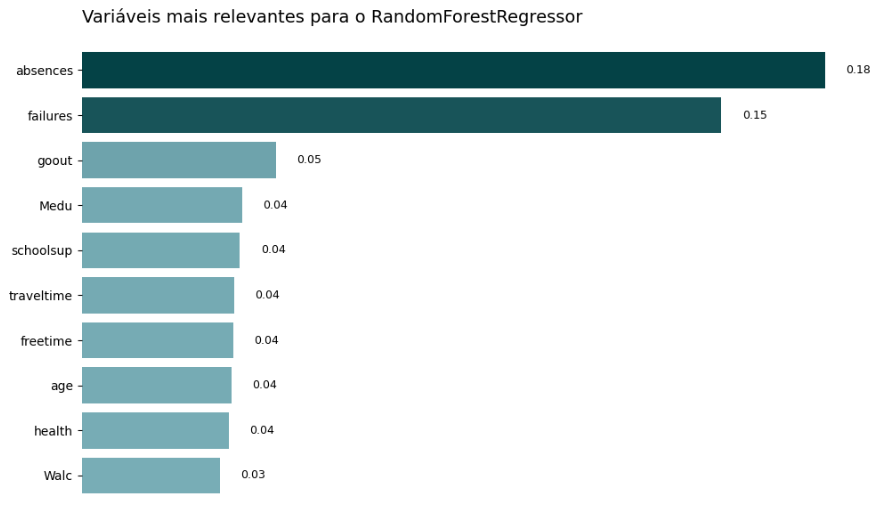
\includegraphics[keepaspectratio]{imagens/grafico_imp_vrs.png.png}}

Frequência - Distribuição.

Relação entre presença e pontuação.

Relevância dos parâmetros no modelo.

\bookmarksetup{startatroot}

\chapter{Resultados}\label{resultados}

Os resultados do modelo Random Forest aplicado ao problema de regressão
foram os seguintes:

\pandocbounded{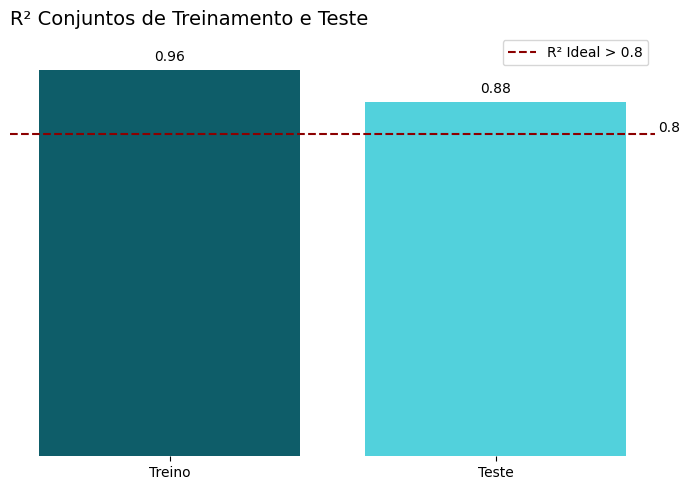
\includegraphics[keepaspectratio]{imagens/metrics.png}}

Média R2: 0.82 MAE: Indicador de baixa precisão média. MSE: Também
dentro de uma faixa tolerável, melhorando a precisão das previsões.

Esses achados corroboram a hipótese inicial: existe uma correlação
significativa entre a presença dos estudantes e suas notas.

Principais Percepções:

A presença na escola é um forte indicador do rendimento acadêmico. A
automatização do registro de presença pode oferecer informações valiosas
para as instituições educacionais. O modelo criado é capaz de antecipar
com acurácia as notas dos estudantes com base na sua frequência.

Essas percepções foram cruciais para demonstrar aos interessados a
viabilidade da implementação do sistema RFID.

\bookmarksetup{startatroot}

\chapter{Conclusão}\label{conclusuxe3o}

Estas são as principais conclusões, dificuldades enfrentadas, próximos
passos e sugestões

Este projeto evidenciou, através da análise de dados e do aprendizado de
máquina, uma ligação direta entre a frequência escolar e o rendimento
acadêmico.

A elaboração de um modelo preditivo com base em Random Forest obteve
êxito, explicando 82\% da variação das notas dos estudantes.

Para além dos resultados da modelagem, o sistema RFID se apresenta como
uma solução eficaz para:

Melhorar a gestão de presença. Coletar automaticamente informações para
análises futuras. Suportar a administração acadêmica de maneira eficaz.
Proximos passos sugeridos:

Criação de um modelo experimental do sistema RFID. Coleta de dados reais
de presença por RFID para aprimoramento do modelo. Ampliação da análise
incorporando outros elementos, tais como envolvimento em atividades,
rendimento em avaliações constantes e histórico acadêmico.

Assim, o projeto cumpre sua função inicial de validar tecnicamente a
importância do controle de presença automatizado para o avanço
acadêmico.

\bookmarksetup{startatroot}

\chapter{Referências}\label{referuxeancias}

As referências estão organizadas no arquivo \texttt{.bib} e serão
exibidas automaticamente.

\phantomsection\label{refs}




\end{document}
